\chapter{Introduction}
\label{ch:introduction}

The Standard Model of Particle Physics (SM) is a quantum field theory (QFT) describing strong and electroweak (EW) interactions.
It was formulated in his current form in the mid-70s and has been an extremely successful and predictive theory since then.
Almost all known phenomena from 1~eV up to almost 200~GeV are well described by the SM and experiments at the Large Hadron
Collider (LHC) are now probing the SM up to the TeV scale.
Finally, in 2013 we were able to observe the Higgs boson, one of the fundamental building blocks of the theory,
giving a solid theoretical basis to it. However, experimentally well established effects, like neutrino
oscillations and the presence of dark matter, are outside the reach of the SM. Furthermore, the model does not include
the description of gravity. Therefore this motivates the search for New Physics (NP).

\begin{table}[h!]
\begin{tabular}{|c|c|c|c|c|}
Interaction	& Mediator	& Rel. strength	& Range	(m)	& Mediator mass (GeV/c${}^2$) \\
\hline
Strong		& $g$		& 1			& $\infty$		& 0		\\
EM			& $\gamma$	& $10^{-3}$		& $\infty$ 		& 0		\\
Weak		& $Z$, $W^\pm$	& $10^{-16}$		& $10^{-18}$	& $W^\pm = 80.399$ \\
			&		&			&		& $Z_0 = 91.188$	\\
Gravity		& $g^0$ (graviton?) & $10^{-41}$	& $\infty$		& 0		\\
\end{tabular}
\caption{Fundamental forces of nature together with their gauge bosons, relative strengths and range.
Gravity is not included in the SM and the graviton is hypothetical at the current time.}
\label{tab:interactions}
\end{table}

The SM is based on the symmetry groups of strong ($SU(3)_C$) and electroweak interactions ($SU(2)_W \times U(1)_Y$).
The subscripts C, W and Y stand for colour charge, weak isospin and hyper-charge. The Lagrangian describing the
SM results from the application of the principle of invariance under the unitary product group $SU(3) \times SU(2) \times U(1)$,
which reflects conservation laws such as the conservation of electric and strong charge.
The model had then 26 free parameters which are experimentally measured.

Particles included in the SM can be grouped under a few categories depending on their properties and ability to interact with
each other. First of all we can distinguish between fermions (half-integer spin particles) and bosons (integer spin particles).
Fermions constitute the basic building blocks of matter, while bosons are the mediators of the interaction between them.
Since in the SM the concept of bosonic mediators of interactions arises because of gauge symmetry~\cite{Glashow:1961tr},
they are called ``gauge bosons". The list of the known interactions with their force carrier and properties is reported
in Tab.~\ref{tab:interactions}. The matter of which we are made is mainly composed of electrons and protons, which have spin 1/2;
protons are then composed of \uquark and \dquark quarks, which again have spin 1/2. Among fermions one can then consider two smaller
groups: quarks and leptons. Quarks carry colour charge and therefore can interact through the, so called, strong interaction,
while leptons, which do not carry colour charge, are insensitive to it.
For each particle exists a corresponding anti-particle with opposite quantum numbers.
Finally, fermions are divided into three families having similar properties but different masses.
This last structure embedded in the SM is also called flavour structure and it will be the main tool
used in this thesis, a more detailed description of it is given in the next sections.
A schematic view of the fundamental particles in the SM is shown in Fig.~\ref{fig:SMparticles}.
%
\begin{figure}[h]
\centering
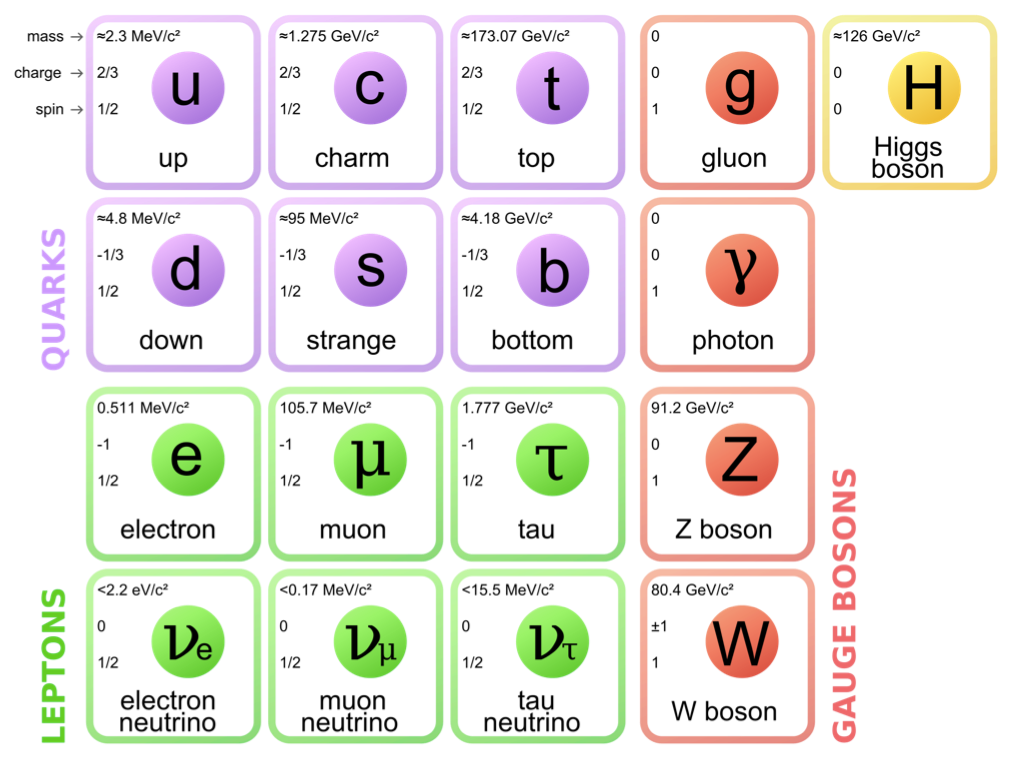
\includegraphics[width=0.7\textwidth]{Introduction/figs/SM.png}
\caption{Diagram of SM particles with their properties.}
\label{fig:SMparticles}
\end{figure}
%
Due to the asymptotic freedom of the strong interaction quarks cannot be observed alone but
are always combined with other quarks to form colour singlets. Non-fundamental particles
composed by quarks are called hadrons and can be divided in mesons, where the color singlet
is achieved by the combination of a quark and its antiquark (\quark\quarkbar), and baryons
formed by three quarks (\quark\quark\quark). 
%Recently evidence for particles composed by 4 quarks was also found~\cite{}.


\section{Electromagnetic and weak interactions}

The Electromagnetic (EM) force is responsible for binding electrons and nuclei together in atoms.
Its force carrier, the photon, is the gauge boson of the EM force. In the SM the photon must be massless,
which also sets the range of the EM force to infinity, since this is proportional to the inverse of the mediator mass.
In fact Heisenberg's Uncertainty Principle tells us that $\Delta E \Delta t > \hbar$, namely virtual particles
of energy $\Delta E$ are allowed to exist for time intervals inferior to $\Delta t$. Thus, since particles can move
at most at the speed of light, $c = 299792458$ ms$^{-1}$~\cite{PDG2014}, this also sets a relation between the length 
of time and space in which a virtual photons can exist ($\Delta t > \hbar / (mc^2)$). As virtual photons can be very
close to the mass shell, this results in a very long lifetime. The EM force has therefore an infinite range.

The weak interaction is responsible for the $\beta$ decay of nuclei. Unlike the electromagnetic force that affects only
charges particles, all known fermions interact through the weak interaction. In the Standard Model this interaction is mediated
by the emission or absorption of $W^\pm$ and $Z$ bosons. The electroweak symmetry is spontaneously broken by the Higgs
field~\cite{Strocchi:1977za} and this causes the $W^\pm$ and $Z$ bosons to become massive (see 
Tab.~\ref{tab:interactions}).
For this reason the weak force has a very short range. Using Heisenberg's Principle together with Einstein's formula 
$\Delta E = m c^2$, which relates mass and energy, and knowing that the maximum space that a particle can cover in a time 
$\Delta t$ is $r = c \Delta t$, qualitatively $r \sim \hbar / mc$. In this picture the carriers of the weak force can travel
$r \sim 2 \cdot 10^{-3}$~fm.
The weak interaction is also the only one that violates parity-symmetry, which states that interactions are invariant under
a reflection of all coordinates. This symmetry breaking arises from the fact that only left-handed fermions interact through
the weak interaction. The first experiment showing this was made by Wu in 1957~\cite{Wu:1957my}. Similarly, the weak interaction
is the only one that also breaks the CP symmetry, which combines parity transformations and ``charge conjugation".
This is particularly interesting because all interactions are invariant under the CPT transformation, which combines the CP
transformation and time reversal, hence, breaking CP the weak interaction must also be not invariant under time reversal.

In 1968 Salam, Glasow and Weinberg unified the weak and electromagnetic forces in a single theory,
having a single coupling constant~\cite{PDG2014}. The EW interactions are divided into charged currents (CC) and neutral
currents (NC). In the first group, quarks and leptons interact with the $W^\pm$ bosons, producing decays such as
$\mu^+(\mu^-) \rightarrow e^+ \nu_e \overline{\nu}_\mu (e^- \overline{\nu}_e \nu_\mu)$ and $n \rightarrow p e^- \overline{\nu}_e (\overline{p} e^+ \nu_e)$.
The study of these processes confirmed that only the left-handed (right-handed) component of fermions (anti-fermions)
takes part in weak processes. The CC interactions have a peculiarity: they are the only interactions in the SM that violate
flavour conservation at tree level (see next section), while any other interaction not conserving flavour has to happen through
loops. The second group of EW interactions, NC, corresponds diagrams mediated by the photon or the $Z$ boson interacting with
a fermion and its anti-fermion.

%The EM theory results from requiring the fermion Lagrangian to be invariant under local gauge transformations.
%The electron and positron free fermionic fields are defined as $\psi(x)$ and $\bar{\psi(x)}$, where x is a relativistic four vector.
%A local gauge transformation can always be written as:
%
%\begin{align}
%\psi(x) \rightarrow \psi(x') = e^i{\alpha(x)}\psi(x)
%\end{align}
%
%where $\alpha(x)$ can be any function of space and/or time. The free fermion Lagrangian, given by
%
%\begin{equation}
%\mathcal{L} = -i \bar{\psi(x)} \gamma^mu \partial_\mu \psi(x) - m\bar{\psi(x)} \psi
%\end{equation}
%
%is not invariant under such transformations. Greek indices denote space-time directions and imply summation and $\gamma^i$ are the Dirac matrices. If we apply the local gauge transformation and we subtract the initial Lagrangian we get a remaining term
%
%\begin{equation}
%\Delta \mathcal{L} = \mathcal{L}' - \mathcal{L} = -i \bar{\psi}  \gamma^mu \psi \partial_\mu \alpha(x)
%\end{equation}
%
%In order to make the Lagrangian invariant we can introduce a vector field $A$, which transforms as described by Eq. \ref{gauge invariance},  to %compensate for the remaining term: this is the photon field.
%
%\begin{equation}
%\label{gauge invariance}
%A'_\mu = A_\mu -\frac{1}{e}\partial_\mu \alpha(x)
%\end{equation}
%
%Redefining then the field derivative $D_\mu = \partial_\mu - ieA_\mu$, we obtain the invariant Lagrangian:
%
%\begin{equation}
%\mathcal{L} = -i \bar{\psi(x)} \gamma^mu D_\mu \psi(x)  - m\bar{\psi(x)} \psi = -i \bar{\psi(x)} (\gamma^mu \partial_\mu  - m)\psi(x) + e\bar{\psi}  \gamma^mu \psi A_\mu
%\end{equation}





\section{Flavour and the CKM matrix}
\label{sec:flavour}

``Flavour" in particle physics refers to the quark/lepton composition of a particle. The introduction of flavour quantum numbers
was motivated in order to explain why some decays, although kinematically allowed, have never been observed. To all leptons is
assigned a quantum number $L_\ell = 1$ (where $\ell = e,\mu,\tau$), which in the SM is conserved by all interactions.
This conservation is experimentally well established; for example decays like $\mu^- \rightarrow e^- \gamma $, which
is kinematically possible, have never been observed. This is explained by the fact that the lepton number in the initial
and final state are different and therefore lepton flavour is violated.

In the hadronic sector particles carry flavour numbers described as follow:

 \begin{itemize}
 \item \emph{Isospin}: $I_3 = 1/2$ for the up quark and value $I_3 = -1/2$ for the down quark;
 \item \emph{Strangeness}: $S = -(n_s - \bar{n}_s)$, where $n_s$ is the number of strange quarks and $\bar{n}_s$ is the number of anti-strange quarks;
 \item \emph{charmness, bottomness, topness}: in analogy to strangeness
 they are respectively defined as $C = -(n_c - \bar{n}_c)$, $B = -(n_b - \bar{n}_b)$, $T = -(n_t - \bar{n}_t)$.
 \end{itemize}

As mentioned before, in the SM the only interaction violating flavour conservation is the weak interaction
when mediated by $W^\pm$ bosons.

Measuring branching fractions of weak decays like $\pi \to \mu \nu_\mu$ and $K \to \mu \nu_\mu$, corresponding
respectively to $ud\to\mu\nu_\mu$ and $us\to\mu\nu_\mu$ processes, suggested the existence of more than one
coupling constant for different quarks. Cabibbo~\cite{PDG2014}, in order to preserve the universality
of weak interactions, suggested that the branching fraction differences could arise from the fact that
the doublets participating in the weak interactions are an admixture of the flavour eigenstates. He therefore introduced
the Cabibbo angle, $\theta_c$, considering that eigenstates participating to the weak interaction are rotated with respect
of the flavour eigenstates.

\begin{equation}
\left( \begin{array}{c}
d_W \\ s_W
\end{array} \right) =
\left( \begin{array}{cc}
\cos \theta_c  & \sin \theta_c\\
-\sin \theta_c & \cos \theta_c
\end{array} \right)
\left( \begin{array}{c}
d \\ s
\end{array} \right) = 
\left( \begin{array}{c}
\cos\theta_c \cdot d + \sin \theta_c \cdot s \\
\cos \theta_c \cdot s - \sin \theta_c \cdot d
\end{array} \right)
\end{equation}

Considering a 6 quark system one angle is not enough to describe a rotation but the mixing system can be generalised
using a $3 \times 3$ unitary matrix, which is called CKM matrix, from the names of Cabibbo, Kobayashi and Maskawa.
The unitarity of the matrix is required preserved the universality of the weak interaction. Theoretically, a $N \times N$ complex
matrix is dependent on $2 \cdot N^2$ real parameters. Requiring unitarity ($AA^\dagger = A(A^*)^T = I$), the number
of independent parameters left is $(N - 1)^2$. Therefore a $3 \times 3$ matrix depends then on 4 real parameters, which
can be divided in 3 real constants and one imaginary phase. The imaginary phase generates the CP-violation which was
observed in weak interactions. In Eq.~\ref{CKM} is reported a parametrisation of the CKM matrix together with the most
recent measured values of its terms~\cite{PDG2014}. In this parametrisation $\rho$, $A$, and $\lambda$
are the real constants and $\eta$ the imaginary phase; in Eq.~\ref{params} are reported their relations with the 3 mixing angles.
%
\begin{multline}
V_{CKM} = \left( \begin{array}{ccc}
1 - \lambda^2/2 & \lambda  & A \lambda^3(\rho -i\eta) \\
-\lambda & 1 - \lambda^2/2 & A\lambda^2 \\
A \lambda^3(1 - \rho -i\eta) & A\lambda^2 & 1 
\end{array} \right) + O(\lambda^3)= \\
= \left( \begin{array}{ccc}
0.97427 \pm 0.00015 & 0.22534 \pm 0.00065 & 0.00351^{+0.00015}_{-0.0014} \\
 0.22520 \pm 0.00065 & 0.97344 \pm 0.00016 & 0.00412^{+0.0011}_{-0.0005} \\
 0.00867^{+0.00029}_{-0.00031} & 0.0404^{+0.0011}_{-0.0005} & 0.999146^{+0.000021}_{-0.000046} \\
\end{array} \right)
\label{CKM}
\end{multline}
%
\begin{align}
\lambda & = \sin(\theta_{12}) = \sin(\theta_c) \\
A\lambda^2 & = \sin(\theta_{23}) \\
A\lambda^3(\rho - i\eta) & = \sin(\theta_{13})e^{i\delta}
\label{params}
\end{align}
%
\begin{figure}[h!]
\centering 
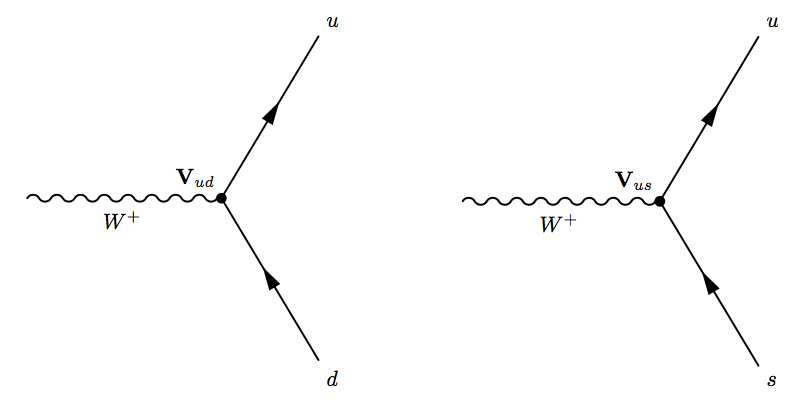
\includegraphics[width=0.6\textwidth]{Introduction/figs/ch_currents_ckm.png}
\caption{Feynman diagrams with CKM weights on weak interaction vertices}
\label{fig:ch_currents_ckm}
\end{figure}
%
Figure~\ref{fig:ch_currents_ckm} displays examples of CC processes together with the CKM elements associated with their vertices.
It is interesting to note that the CKM matrix has a hierarchical form, namely elements on the diagonal are approximately
1 and become smaller and smaller going farther from the diagonal. This structure is not explained in the SM.
Another feature to note is that, due to the unitarity of the matrix, the transformation have no effect on neutral interactions.
In fact defining $q' = Vq$
%
\begin{equation}
\bar{q}'q' = \bar{q}V^{*}Vq = \bar{q}q.
\end{equation}
%
As a result flavour-changing neutral currents are forbidden at tree level in the SM.

As mentioned, the CKM matrix has to be unitary to preserve probability and this imposes constraints to its terms of the form:
\begin{equation}
\sum_i |V_{ik}|^2 = 1 \text{ and } \sum_k V_{ik} V^{*}_{jk} = 0.
\end{equation}
These correspond to a constraint to three complex numbers, which can be viewed
triangles in the $(\rho,\eta)$ plane and are called ``unitarity triangles".
The most commonly used unitarity triangle arises from
\begin{equation}
V_{ud}V^*_{ub} + V_{cd}V^*_{cb} + V_{td}V^*_{tb}=0.
\end{equation}
Figure~\ref{fig:unitarity_triangle} shows a representation of such triangle together with
a plot summarising the most up to date experimental constraints to its parameters~\cite{Charles:2015gya}.
The precise measurement of the parameters of the CKM matrix
is a powerful stability test of the standard model and sets a solid base for new physics
searches in the flavour sector. One of the main goals of the LHCb experiment is to precisely
measure the angle $\gamma$, which is currently the least constrained from measurements.
 %
\begin{figure}[h!]
\centering 
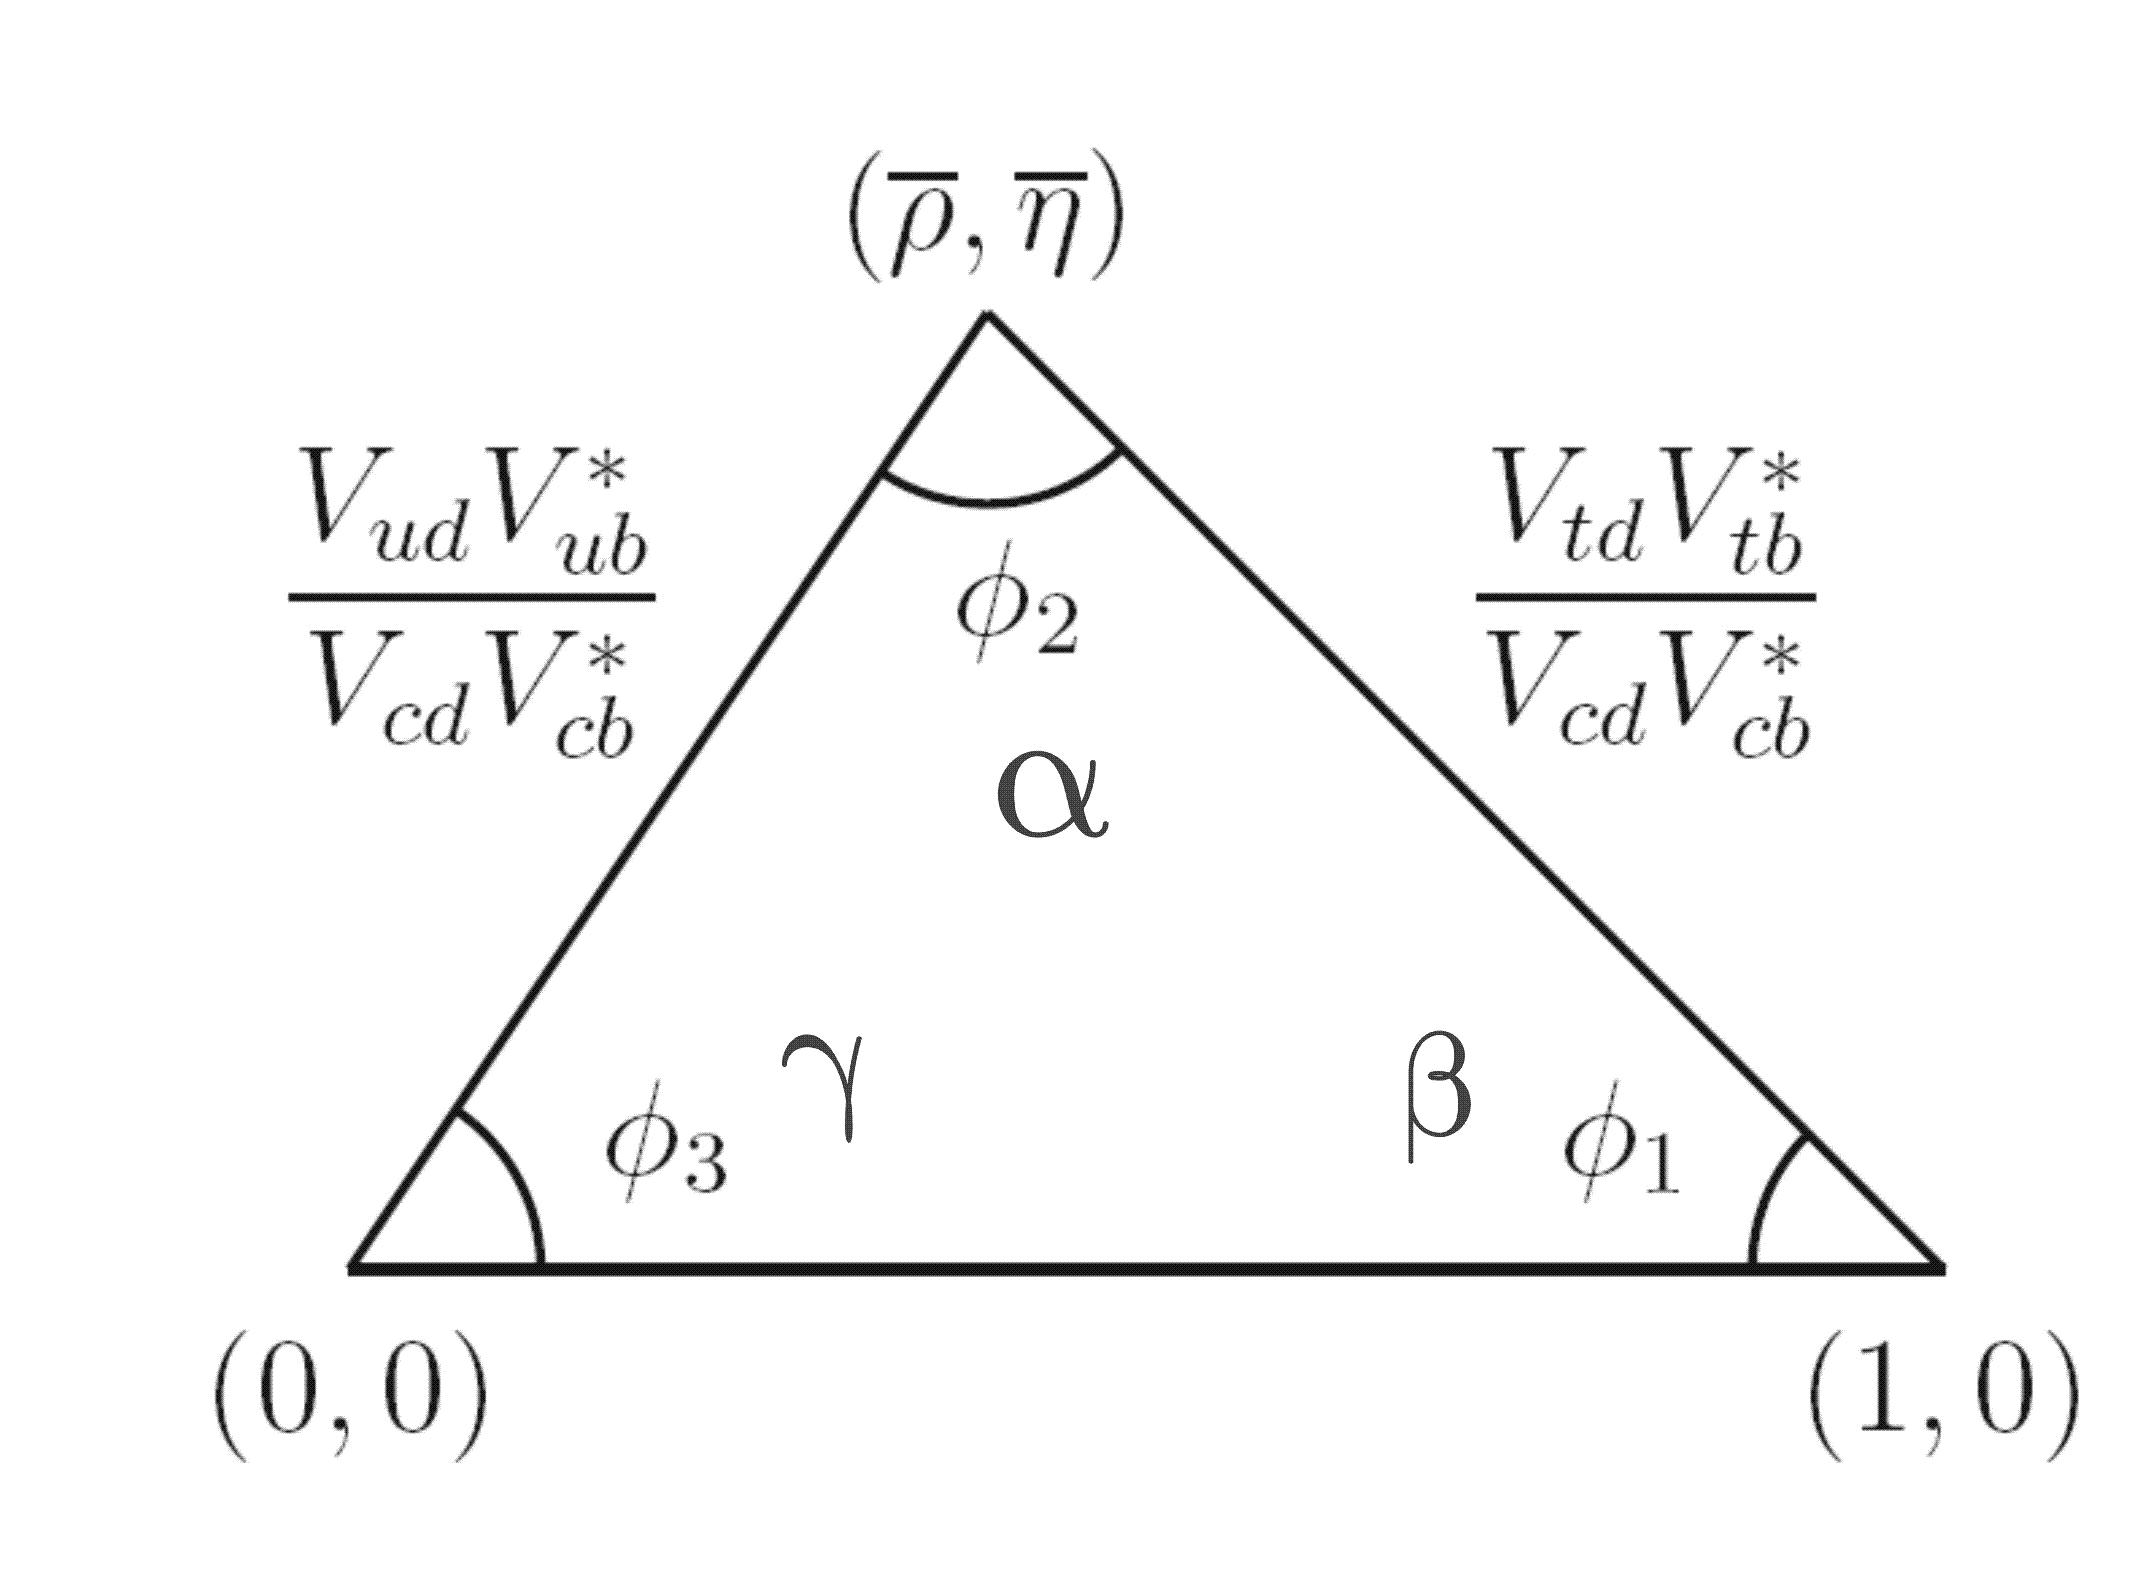
\includegraphics[width=0.6\textwidth]{Introduction/figs/Unitarity_triangle.png}
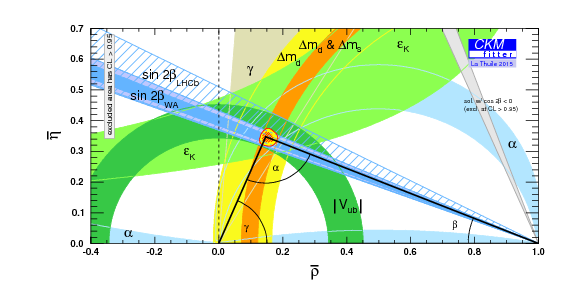
\includegraphics[width=0.9\textwidth]{Introduction/figs/Unitarity_triangle_HFAG.png}
\caption{(top) A representation of the unitarity triangle and its parameters.
(bottom) A summary of the most up to date measurements of the unitarity triangle parameters~\cite{Charles:2015gya}.}
\label{fig:unitarity_triangle}
\end{figure}
 
 
 
 
\section{The puzzles of the SM}
\label{sec:SMproblems}

Despite the confirmation of many predictions of the SM, the theory has several limitations
and is unable to account for some well established experimental facts:
%
\begin{itemize}
\item \emph{Dark matter}: experimental evidence tells us that the content of visible matter in the universe is not enough
to account for the observed rotation of galaxies~\cite{Zwicky:1933gu}. The more natural way to solve the problem
is the hypothesis of a form of matter that interacts with the gravitational field but not with the interaction of the SM. 
%Furthermore, studies of the fluctuations of the cosmic microwave background indicate the existence of
%cold dark matter~\cite{Dunkley:2008ie}.
%formed of particles which do not interact through the SM forces and
%for which there is no SM candidate.
%
\item \emph{Matter-antimatter asymmetry}: a large asymmetry is observed between the quantity of matter and antimatter
in the universe. Assuming that both were equally created in the initial state of the universe, a condition such
as the violation of the CP symmetry is necessary to account for such observed differences. However, the magnitude of
CP violation predicted by the SM is not enough to explain the observed imbalance~\cite{Gavela:1993ts}.
%
\item \emph{Gravity}: even though the gravitational force was the first to be discovered this is not included in the SM.
In fact when introducing gravity in the framework of QFT the theory diverges. On the other hand
gravity becomes irrelevant for small masses as those of particles and can be neglected in good approximation.
Many attempts were made but there is not yet a consistent procedure to introduce gravity in the SM. 
%
\item \emph{Neutrino oscillation}: measurements regarding solar and atmospheric neutrinos as wells as
neutrinos from nuclear reactors established that neutrinos can change flavour while propagating in space.
This is not predicted in the SM, in fact in the SM neutrinos are massless, while an oscillation requires a non
zero mass~\cite{Maltoni:2011zz}.
%
\item \emph{The hierarchy problem}: The mass of a scalar (spin 0) particle, such as the Higgs boson,
suffers from quantum corrections due to the physics above a certain scale. As new physics can appear
anywhere up to the Planck scale, $\sim 10^{19}$~\gev, these corrections can be very large and it would require
a high level of fine-tuning for them to cancel out and give such a small value as the one measured for the
Higgs Mass,  $\sim 126$~\gevcc~\cite{Feng:2013pwa}. 
%This is considered unnatural by many physicists and pushes them
%to look for further motivations.
%
\end{itemize}
%
In conclusion, even though the SM has been very successful in describing the properties of the observed particles
and their interactions so far. However, because of its many puzzles, it is believed only to be part of a more general theory 
or only to be valid up to a certain energy scale. %Many theoretical models expect New Physics (NP) to enter at the TeV scale.

\subsection{The flavour problem}

%As mentioned in Sec.~\ref{sec:flavour}, flavour conservation is well experimentally established but it does not
%have a strong theoretical otivation in the Standard Model.
Flavour Changing Charged Currents (FCCC) that are mediated by the $W^\pm$ bosons are the only sources of flavour changing interaction in the SM and, in particular, of generation changing interactions, where a quark or a lepton of a family transforms
into one of an other family. Another class of processes is the Flavour Changing Neutral Currents (FCNCs), e.g. transitions from a
\bquark quark with charge of 1/3 to a \squark or \dquark with a charge of +2/3. Examples of FCNC transitions in the quark
and lepton sector are shown in Fig.~\ref{fig:neutr_curr}.
%
\begin{figure}[h!]
\centering 
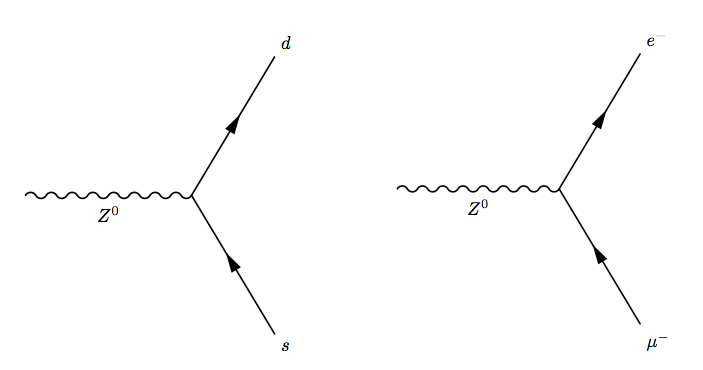
\includegraphics[width=0.6\textwidth]{Introduction/figs/neutral_current_proc.png}
\caption{Feynman diagrams of FCNCs processes forbidden in the SM.}
\label{fig:neutr_curr}
\end{figure}
%
In the SM there is no fundamental reason why
there cannot be FCNCs and, yet, they are experimentally  observed to be highly suppressed.
On the other hand the observation of neutrino oscillation proves that flavour is not an exact symmetry and is not always
conserved. Furthermore, the values of the terms of the CKM matrix and the PMNS matrix,
which the mixing-matrix, equivalent to the CKM, in the lepton sector, are not explained in the SM
and have to be measured experimentally. These open problems motivate searches for flavour symmetries and 
deeper motivations for flavour conservation. 

\section{Beyond the Standard Model}

From the last sections it is evident that, despite the great success of the SM, there is a need to explore new theories. 
Among the most promising approaches there are are those invoking Super-Symmetry and extra-dimensions 
%
In Super-Symmetry new degrees of freedom are introduced to suppress the diverging terms of the scalar mass. This theory
assumes that for each fermion there is a corresponding boson and, since bosons and fermions contribute with opposite
sign to the mass term, these would cancel out~\cite{Fayet:1976cr}. Supersymmetry also provides a natural candidate for dark
matter, the neutralino, which is a weakly interacting stable particle.
%
The idea to introduce extra-dimensions was triggered by the fact that normally gravity is not relevant
in particle physics but it would be natural if all forces had similar strength. By adding extra dimensions to the normal 3 spatial dimensions, one can restore the strength of gravity, as this could be dispersed by the wider space available~\cite{Randall:1999ee}.
%
In all these approaches severe constraints to masses and couplings must be imposed to maintain
compatibility with the SM at the electroweak scale.

\subsection{Flavour and BSM theories}

Most BSM theories predict processes violating flavour conservation. Therefore, the observation or
non-observation of these processes can give important information about new physics.
BSM theories can be classified according to the amount of flavour violation they introduce.
The first class of models to consider is the Minimal Flavour Violation (MFV).
These are models in which the only sources of flavour changing transitions are governed by the
CKM matrix with the CMK phase being the only source of CP violation.
These features can be assured by symmetry principles and these types of models are
naturally compatible with the SM. Examples of such models include the MSSM
which minimal flavour violation and the SM with one extra-dimension. A review of MFV models
is presented in Refs.~\cite{Isidori:2012ts,Buras:2003jf}.
%
The MFV paradigm provides a way to resolve the tension between expectation, driven by naturalness arguments,
that NP should be at the \tev scale and limits on FCNC processes that point to much higher scales.
%
A powerful tests of MFV is provided by the study of ratios between $\bquark\to\dquark$ and $\bquark\to\squark$
transitions, because their hamiltonians share the same structure. One particularly important example is the ratio of
$\Bz$ and $\Bs$ dimuon decay rates~\cite{TomRDreview}, as this is a purely leptonic decay free from hadronic uncertainties.
In the SM such ratios are approximately equal to $|V_{td}/V_{td}| \sim 1/25$, modified by phase space and hadronic
matrix elements, while they can take very different values in non-MFV models.

In the quest for New Physics an important role is also played by simplified models
as a intermediate model building step. Instead of constructing models valid up to the GUT scale
one can consider simplified models, which typically  start from the  SM and incorporate a new sector
with a limited number of parameters. Such models are easier to constrain but can nevertheless point
in the right direction to build more complete theories. The choice of the new sector to add can be driven by the need to
explain existing tensions between data and SM predictions or by theoretical prejudice.
%
Two models especially relevant when studying rare decays are Z'-penguins and leptoquarks.
A Z'-penguin is a FCNC process involving a neutral field arising from an extra U(1) gauge symmetry.
As for the SM penguins, this field contributes in loops causing modifications of the effective couplings
with respect to the SM. A survey of Z' models can be found in Ref.~\cite{Buras:2014zga}.
%
Leptoquarks are bosonic particles that carry one quark and one lepton flavour quantum number.
They can be spin 1 but they are commonly assumed to be scalar particles.
A tree level exchange of a leptoquark induces processes such as $\bquark \to (\squark,\dquark)\ell^+\ell^-$,
and therefore can result in an enhancement of their decay rates with respect to the SM~\cite{Hiller:2014yaa}.
Leptoquarks would also provide a natural explanation for non-universal couplings to leptons,
introducing lepton flavour violation.


\section{Rare decays: a tool to search for new physics}

In the Standard Model FCNC processes are forbidden at tree level but
can occur trough loops diagrams such as \W box or penguin diagrams (see Fig.~\ref{fig:penguins}).
The branching fractions decays going through these processes are small, typically $\sim10^{-6}$ 
or lower, and therefore they are called ``rare decays". Additional NP contributions to the virtual loops
are not necessarily suppressed with respect to the SM component and this makes these decays
very sensitive to new physics. This approach to new physics searches is interesting as
new particles could be at a high mass scale not accessible at colliders but its effect
could be observed in loop effects.
Radiative and penguin decays are particularly interesting because they are theoretically
well understood, which allows precise comparisons with measurements. Finally, they provide
a great quantity of observables that can be affected by NP, not only decay rates, but also CP asymmetries and angular observables such as forward-backward asymmetries. The joint
analysis of different observables can help building a consistent picture and rule out specific models.
%
\begin{figure}[h!]
\centering
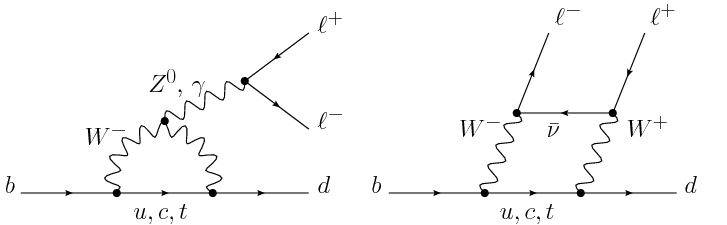
\includegraphics[width=0.8\textwidth]{Introduction/figs/penguin_general.png}
\caption{Loop Feynmann diagrams allowing $\bquark \to \dquark$ FCNC 
processes: penguin diagram (left) and \W box (right).}
\label{fig:penguins}
\end{figure}

\subsection{Theoretical framework: the effective Hamiltonian}
\label{sec:Effective_Hamiltonian}

Rare decays of \bquark hadrons are governed by an interplay between weak
and strong interactions.
%The QCD corrections that arise from hard gluon exchange bring large logarithms
%of the form $\alpha_s^n(m_b)\log^m(m_b/M)$, where $M = m_t$ or $M = m_W$.
%A suitable framework to achieve the necessary resummation of these logarithms
%in an effective low-energy theory with five quarks.
%The QCD corrections that arise from hard gluon exchange bring large contributions
%large logarithms of the form $\alpha_s^n(m_b)\log^m(m_b/M)$, where $M = m_t$ or $M = m_W$.
The large masses of W, Z and top quark compared to that of the \bquark quark allow
the construction of an effective theory divides the the problem of calculating
weak decay amplitudes into two parts, The first part deals with ``short distance" physics, namely
perturbative contributions due to energy scales above the \bquark mass. The second parts handles
 ``long distance", typically non-perturbative, contributions. Figure~\ref{fig:fermi_theory} illustrates 
an example of a Fermi theory where the short distance physics is hidden into a point like vertex.
\begin{figure}[h!]
\centering
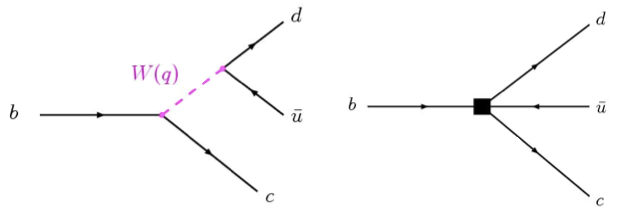
\includegraphics[width=0.8\textwidth]{Introduction/figs/fermi_theory.png}
\caption{Example of a Fermi theory in which the full theory is divided between the
short distance contribution, hidden in the vertex, and the long distance contribution.}
\label{fig:fermi_theory}
\end{figure}
The effective hamiltonian~\cite{Chetyrkin:1996vx} of such a theory relevant to
$\bquark\to\squark/\dquark \gamma$ and  $\bquark\to\squark/\dquark \ell^+\ell^-$
transitions can be written as:
%
\begin{equation}
\mathcal{H}_{eff} = \frac{-4G_F}{\sqrt{2}} \left[ \lambda^t_q \sum C_i(\mu,M)\mathcal{O}_i(\mu)
+ \lambda^u_q \sum C_i(\mu,M)(\mathcal{O}_i(\mu) - \mathcal{O}_i^u(\mu)) \right]
\end{equation}
%
where $G_F$ denotes the Fermi coupling constan and the $\lambda$ constants are the CKM factors,  $\lambda^t_q = V_{tb}V_{tq}^*$ and  $\lambda^u_q = V_{ub}V_{uq}^*$. To obtain this formula the method of the Operator Product Expansion (OPE)~\cite{Buchalla:1995vs} was used to allow the separation into
the long-distance contributions, contained in the operator matrix elements, $\mathcal{O}_i$, and the short-distance physics described by the so called Wilson Coefficients, $C_i$.
Operators and coefficient are evaluated at the renormalization scale $\mu$.
In $\bquark\to\squark$ quark transitions, which are the main topic of this thesis, 
the doubly Cabibbo-suppressed contributions proportional to $\lambda^u_s$ can be neglected.

In order to describe SM processes the effective theory must be matched
with the SM at the EW scale, $\mu_W$,. Then, using the scale independence of the
effective hamiltonian, one can derive a renormalization group equation for the Wilson Coefficients
%
\begin{equation}
\mu \frac{\deriv}{\deriv \mu} C_i(\mu) = \gamma_{ij}C_j(\mu)
\end{equation}
%
where the matrix $\gamma$ is the anomalous dimensions matrix of the operators $\mathcal{O}_i$.
At leading order the solution is given by~\cite{Buras:1998raa}:
%
\begin{equation}
C_i(\mu) = \left[ \frac{\alpha_s(\mu_W)}{\alpha_s(\mu)}\right]^{\frac{\gamma^0_{ii}}{2\beta_0}} C_i(\mu_W) = \left[ \frac{1}{1 + \beta_0\frac{\alpha_s(\mu)}{4\pi}ln\frac{\mu_W^2}{\mu^2}} \right]^{\frac{\gamma^0_{ii}}{2\beta_0}} C_i(\mu_W)
\end{equation}
%
where $\alpha_s$ is the strong coupling constant. In the SM at $\mu_s = m_b$ the
Wilson Coefficients have values:
%
\begin{equation}
\begin{array}{ccc}
C_7^{SM} = -0.3, & C_9^{SM} = 4.2, & C_{10}^{SM} = -4.2.
\end{array}
\end{equation}
%
New physics contributions appears in the Wilson Coefficients in the form of additive factors:
 $C_i = C_i^{NP} + C_i^{SM}$.

Finally, the amplitudes of exclusive hadronic decays can be calculated as the expectation 
values of the effective hamiltonian. Given an initial state $I$ and a final state $F$
(e.g. $I = B$ and $F=\Kstarz\mumu$) they can be calculated as
%
\begin{equation}
A(M\to F)= \langle M | \mathcal{H}_{eff} | F \rangle = 
\mathcal{H}_{eff} = \frac{G_F}{\sqrt{2}} \sum V_{CKM}^i C_i(\mu) \langle M | \mathcal{O}_i(\mu) | F \rangle
\end{equation}
where $\langle M | \mathcal{O}_i(\mu) | F \rangle$ are the hadronic matrix elements also called  ``form factors".
These can be evaluated using non perturbative methods such as lattice calculations.
However, due to the limitations of these methods, the dominant theoretical uncertainties
reside in the calculation of the matrix elements.

\subsection{Operators}
\label{sec:operators}

Separating the left- right-handed components the relevant effective Hamiltonian
for $\bquark\to\squark\ell^+\ell^-$ transitions is
%
\begin{equation}
\mathcal{H}_{eff} = \frac{4G_F}{\sqrt{2}} V_{tb}V^*_{ts} \frac{\alpha_e}{4\pi} \sum_{i=1}^{10} \left[ C_i \mathcal{O}_i  +  C'_i \mathcal{O}'_i \right].
\end{equation}
%
%where the $V_{ub}$ and $V_{bs}$ are the factors of the CKM matrix.
The operators are that are important for electroweak penguin processes are the following~\cite{TomRDreview}:
%
\begin{equation}
\begin{array}{ll}
 \mathcal{O}_7 = \frac{m_b}{e} (\bar{s} \sigma^{\mu\nu}P_Rb)F_{\mu\nu}  		& \mathcal{O}_7' = \frac{m_b}{e} (\bar{s} \sigma^{\mu\nu}P_Lb)F_{\mu\nu} \\
\mathcal{O}_8 = g_s\frac{m_b}{e} (\bar{s} \sigma^{\mu\nu}P_RT^ab)G^a_{\mu\nu}  	& \mathcal{O}_8' = g_s\frac{m_b}{e} (\bar{s} \sigma^{\mu\nu}P_LT^ab)G^a_{\mu\nu} \\
\mathcal{O}_9 = (\bar{s} \gamma_{\mu}P_Lb)(\bar{\ell}\gamma^\mu\ell) 			& \mathcal{O}_9' = (\bar{s} \gamma_{\mu}P_Rb)(\bar{\ell}\gamma^\mu\ell) \\
\mathcal{O}_{10} = (\bar{s} \gamma_{\mu}P_Lb)(\bar{\ell}\gamma^\mu\gamma_5\ell) 	& \mathcal{O}_{10}' = (\bar{s} \gamma_{\mu}P_Rb)(\bar{\ell}\gamma^\mu\gamma_5\ell)
\end{array}
\end{equation}
%
where $P_{L/R} = (1 \mp \gamma_5)/2$ denotes the left/right handed chiral projection,
$T^a$ are the QCD generators and $F_{\mu\nu}$ ($G_{\mu\nu}$) is the electromagnetic
(chromo-magnetic) field tensor.
%
The $\mathcal{O}'$ operators correspond to right-handed coupling obtained by swapping
$P_R$ and $P_L$ in the equations. In the SM, as well as in MFV models where the
flavour violation is entirely ruled by the CKM matrix, the results $C'$ Wilson Coefficients 
are suppressed by the strange coupling $C'_i \sim (m_s / m_b) C_i$.
%
The operator $\mathcal{O}_7$ is the dominant contribution to the radiative 
$\bquark\to\squark\gamma$ transitions, while $\mathcal{O}_9$ and $ \mathcal{O}_{10}$
are the dominant contributions in semileptonic $\bquark\to\squark\ell^+\ell^-$ decays.
The vertices corresponding to these operators are shown in Fig.~\ref{fig:vtx_operators}
%
\begin{figure}[h!]
\centering
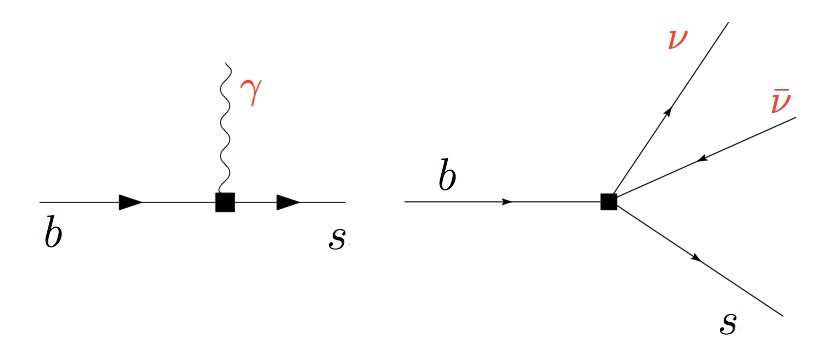
\includegraphics[width=0.6\textwidth]{Introduction/figs/vtx_operators.png}
\caption{Interaction vertices corresponding to the radiative (left) and semileptonic (right) operators.}
\label{fig:vtx_operators}
\end{figure}

It is also common to express the semileptonic operators in a basis with left and right projected leptons
%
\begin{equation}
\begin{array}{ll}
\mathcal{O}_{LL} = ( \mathcal{O}_{9} - \mathcal{O}_{10})/2 & \mathcal{O}_{LR} = ( \mathcal{O}_{9} + \mathcal{O}_{10})/2 \\
\mathcal{O}_{RR} = ( \mathcal{O}'_{9} - \mathcal{O}'_{10})/2 & \mathcal{O}'_{RL} = ( \mathcal{O}'_{9} + \mathcal{O}_{10})/2 \\
\end{array}
\end{equation}
%
where the Wilson Coefficients are also redefined as
\begin{equation}
\begin{array}{ll}
C_{LL} = C_{9} - C_{10} & C_{LR} =  C_{9} + C_{10} \\
C_{RR} = C'_{9} - C'_{10} &C'_{RL} =  C'_{9} +C_{10} \\
\end{array}
\end{equation}
%
This basis is particularly useful in frameworks where BSM physics at a high mass scale
respects the SU(2)$_L$ part of the SM gauge symmetry group.
For instance, instead of fitting the two parameters $C_9$
and $C_{10}$, the LL-hypothesis gives the constraint $C_9 + C_{10} = 0$.

Finally, in the picture presented in this section all operators were considered as universal
with respect of the flavour of the involved leptons. However, BSM models often contain courses of
lepton flavour violation leading to a split of the same operators into two groups depending on the lepton considered. 

\subsection{Phenomenology of $\bquark\to\squark\ell^+\ell^-$ decays}
\label{sec:theo_qsq}

Semileptonic \bquark hadron decays are characterised by two kinematic regimes which
are treated theoretically in different ways: at low \qsq, where the emitted hadron is energetic 
($E > \Lambda_{QCD}$ in the \bquark hadron rest frame), the QCD factorisation applies;
at high \qsq, the region of low hadron recoil ($\qsq = O(m_b)$), an Operator Product Expansion
in $1/m_b$ is valid. In both regions decay rates can be predicted using the different methods and
the biggest uncertainties come from the limited knowledge of hadronic transition matrix elements.
%
\begin{figure}[h!]
\centering
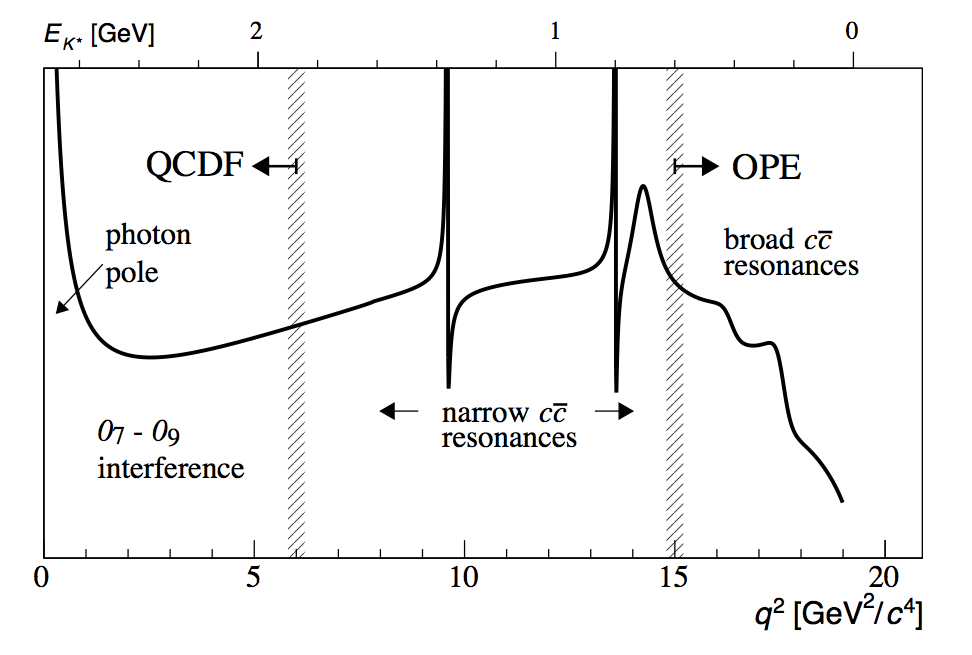
\includegraphics[width=0.8\textwidth]{fig/q2spectrum.png}
\caption{A typical $q^2$ spectrum of $\bquark\to\squark\ell^+\ell^-$ process characterised by the pho
ton pole
at very low \qsq, charmonium resonances at central \qsq and broad resonances at high \qsq.}
\label{fig:q2spectrum}
\end{figure}
%
As can be seen in Fig.~\ref{fig:q2spectrum} the very low \qsq is characterised by a peak due
to the virtual photon contribution, associated with $C_7$. In the region $1-6$ \gevgevcccc the 
interference between $C_7$ and $C_9$ becomes large, yielding sensitivity to NP in $C_9$.
The $6-15$ \gevgevcccc interval is dominated by the charmonium resonances, \jpsi and \psitwos,
though the tree level $b\to\cbar c s$ transition. Although the decays can be experimentally vetoed in
principle charmonia affect the entire \qsq space. Finally, at high \qsq broad charmonium resonances can contribute, like those observed by LHCb in $\decay{B^+}{K^+\mumu}$ decays~\cite{LHCB-PAPER-2013-039}.

\subsection{Observables in $\bquark\to\squark\ell^+\ell^-$ decays}
\label{sec:observables}

Rare decays and especially semileptonic $\bquark\to\squark\ell^+\ell^-$ processes offer a number
of observables which can be used to benchmark BSM models.
The most direct effects appear in decay rates that can be enhanced by NP but the precision on
these measurements is often limited by the uncertainty on form factor calculations.
Therefore, it is important to also look for different observables.
One important class of observables are angular quantities that can often carry complementary 
information about NP with respect to branching ratio measurements. The most basic of these
observable are forward-backward asymmetries that characterise the angular distribution of final particles. 
For the $\Bz\to\Kstar\mumu$ decay combinations of observables have been proposed
that are independent of form factor uncertainties at leading order order~\cite{TomRDreview}.

One way to build safe observables is to construct ratios between similar
decays, in which uncertainties due to the hadronization process cancel out.
These observables include the $R_H$ ratios, between \Bz decay into electrons and muons,
that are described in detail in Sec.~\ref{sec:RKst_theory}.
It is also interesting to compare decays which go though the same fundaments process but
where the spectator quark has a different flavour. This is the case of $\Bu\to K^+\mumu$ and $\Bz\to\KS\mumu$
decays, which are both $\bquark\to\squark$ transitions where the spectator quark is an \uquark quark
in the first case and a \dquark quark in the second. The ratio of the branching fractions of these
decays is called isospin asymmetry.


\section{Experimental status}

To set the background for the searches included in this thesis, this section reports a review
of recent results of NP searches involving rare decays or lepton flavour violation.
Among these, results recently obtained by the \lhcb experiment show a series of anomalies
with respect to the SM that have the potential to yield to NP scenarios.


\subsection{Dimuon decays of \bquark hadrons}

Decays of $B$ mesons into two muons have been recently studies at the \lhcb and \cms experiments.
These are two-body decays where the two muons are back to back in the hadron rest frame.
The simple signatures of these decays makes them easy to study and the fact that they
are unaffected by hadronic physics in the final state makes predictions very clean and precise.
Therefore these are essential tests of the SM.
The $\decay{\Bz}{\mumu}$ and $\decay{\Bz}{\mumu}$ decays are exceedingly rare in the SM.
First of all they are FCNCs that can only happen in loops and furthermore they are CKM-suppressed.
In addition to that the decay of a pseudo-scalar $B$ meson into two muons has a significant helicity
suppression. The latest SM predictions for these decay rates are~\cite{Bobeth:2013uxa}:
%
\begin{align}
\mathcal{B}(\decay{\Bs}{\mumu}) &= (3.65 \pm 0.23) \times 10^{-9} \text{ and } \\
\mathcal{B}(\decay{\Bz}{\mumu}) &= (1.06 \pm 0.09) \times 10^{-10}.
\end{align}
%
The uncertainties on these values mainly come from the knowledge of the decay constants and 
CKM-elements. BSM models can produce significant enhancement to these decay rates.
Furthermore, the measurement of their ratio is a stringent test of the MFV hypothesis.
A combination of the \lhcb and \cms results measured the values~\cite{CMS:2014xfa}:
%
\begin{align}
\mathcal{B}(\decay{\Bs}{\mumu}) &= (2.8^{+0.7}_{-0.6}) \times 10^{-9} \text{ and } \\
\mathcal{B}(\decay{\Bz}{\mumu}) &= (3.9^{+1.6}_{-1.4}) \times 10^{-10}.
\end{align}
%
Both decays where previously unobserved and now the $\Bs$ decay was observed
with a significance of $6\sigma$ and evidence for the $\Bz$ decay was found
with a $3\sigma$ significance. These are compatible with SM predictions within 
$2\sigma$ and put strong constraints to the available parameter-space for BSM 
theories. Figure~\ref{fig:bsmumu} shows the fit the dimuon invariant mass
of $B$ meson candidates where the peaks of the two decays are visible.
%
\begin{figure}[h!]
\centering
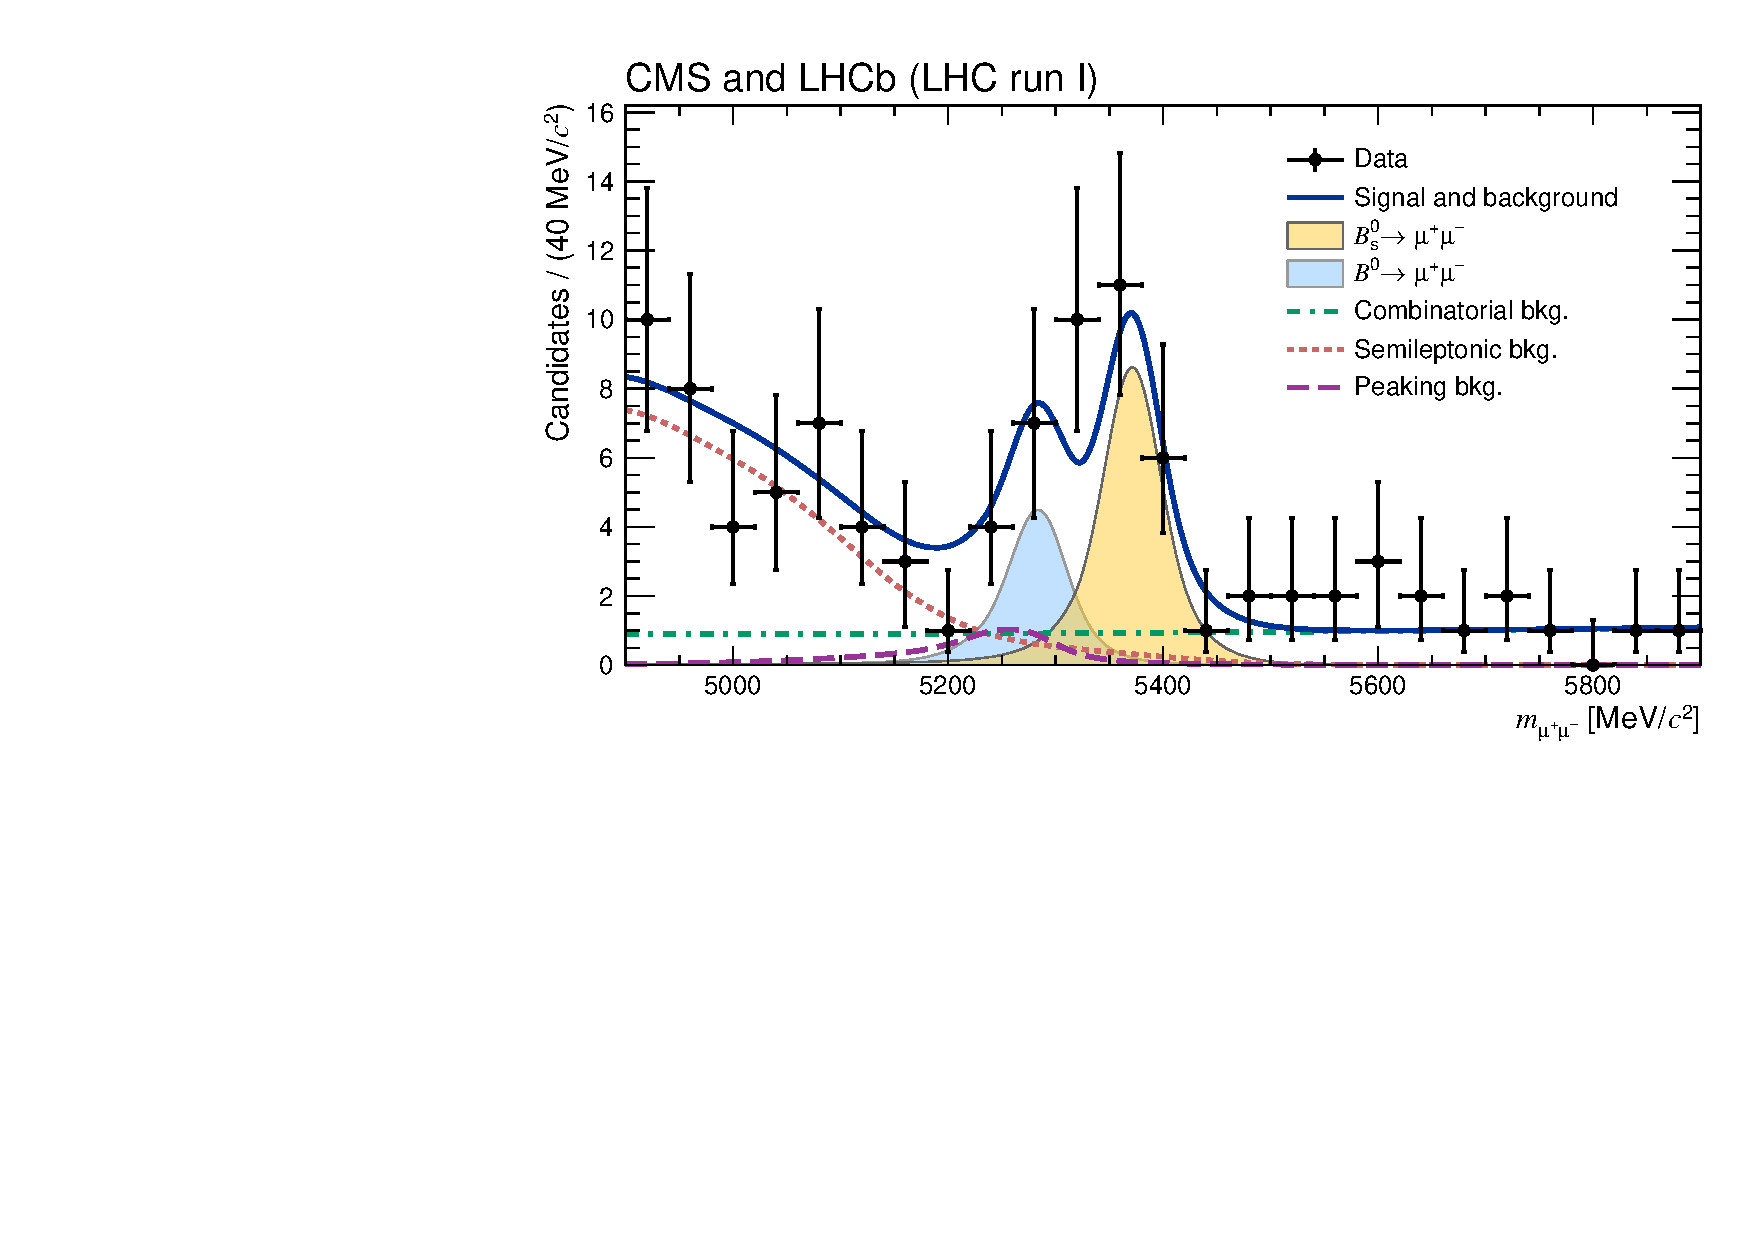
\includegraphics[width=0.6\textwidth]{Introduction/figs/CMSLHCb_EDfig2.pdf}
\caption{Dimuon invariant mass of $B$ candidates showing peaks corresponding 
$\Bs\to\mumu$ and $\Bz\to\mumu$ decays~\cite{CMS:2014xfa}.}
\label{fig:bsmumu}
\end{figure}


\subsection{Semileptonic $\bquark\to\squark\ell^+\ell^-$ decays}

At the LHC energies is now possible to collect large data sample of semileptonic 
decays, especially those with a dimuon pair in the final state.
Many branching fractions of semileptonic $B$ meson decays were recently measured at
the \lhcb experiment, including $\decay{B}{K\mumu}$, $\decay{B}{\Kstarz\mumu}$
and $\decay{\Bs}{\phi\mumu}$~\cite{LHCB-PAPER-2013-017,LHCB-PAPER-2013-019,Aaij:2014pli}. 
Baryon decays where also studied at \lhcb: including the branching fraction of
the rare $\decay{\Lambda_b}{\Lz\mumu}$ decay~\cite{Aaij:2015xza}, which is described in this thesis.
Unlike for pure leptonic decays, SM predictions for semileptonic decays are affected by the
knowledge of hadronic form factors, which yields in relatively large uncertainties,
$\mathcal{O}(30\%)$. As a result measurements are now typically more precise than predictions.

As described in Sec.~\ref{sec:observables} angular observables can be affected by 
new physics. Particular interest was risen by the measurement of a series of observables in
$\decay{B}{\Kstarz\mumu}$ decays, free from form factors uncertainties at leading order~\cite{LHCB-PAPER-2013-037}.
%
\begin{figure}[h!]
\centering
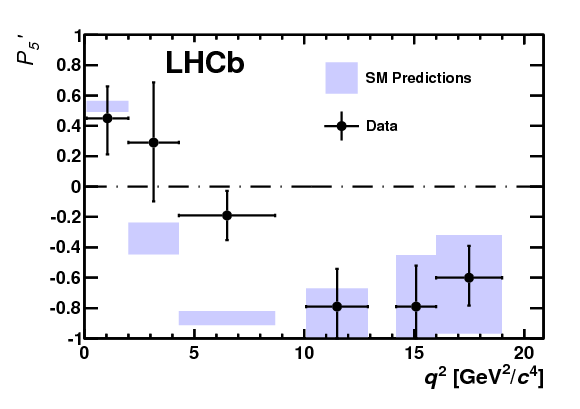
\includegraphics[width=0.7\textwidth]{Introduction/figs/P5prime.png}
\caption{Measurement of the observable as a function of \qsq, showing a tension with
SM predictions in the 2--6 \gevgevcccc region.}
\label{fig:P5prime}
\end{figure}
%
Most of the measurements are found to be in agreement with SM predictions
with the exception of the $P'_{5}$ observable, shown in Fig.~\ref{fig:P5prime}, which presents
a local $3.7\sigma$ deviation. Attempts to build a consistent picture point to a NP contribution
to the Wilson Coefficient $C_9$~\cite{Descotes-Genon:2013wba}.
An angular analysis of $\Bu\to K^+\mumu$ decays was also performed, where observables
are found to be compatible with SM predictions~\cite{LHCB-PAPER-2014-007}.

Other observables for which the sensitivity to form factors effects is reduced are the CP asymmetry between
$B$ and $\bar{B}$ decays, $\mathcal{A}_{CP}$, and the isospin asymmetry between \Bz ad \Bu decays.
Due to the small numerical size of the corresponding CKM elements CP asymmetries of $\Bz\to K^{(*)}\mumu$
decays are tiny in the SM, $O(10^{-3})$. In BSM models new sources of CP violation can arise and therefore
their measurement is a powerful null test of the SM. 
The isospin asymmetry, $\mathcal{A}_{I}$, between \Bu and \Bz is not zero in the SM due
to isospin breaking effects in the form factors.
This is expected to be $\sim1$\% at low \qsq and grow up to $\sim1$\% as \qsq tends to zero.
The LHCb experiment, using the full dataset collected in Run I, corresponding to an integrated luminosity of
3 \invfb measured both these asymmetries to be consistent with zero~\cite{LHCB-PAPER-2014-006,LHCB-PAPER-2014-032}, as reported in Tab.~\ref{tab:AcpAI}. 
%
\begin{table}
\begin{small}
\begin{tabular}{l|cc|cc}
					& \multicolumn{2}{c|}{$\Bz\to K^+\mumu$}			&\multicolumn{2}{c}{$\Bz\to \Kstarz\mumu$}	\\
\qsq [\gevgevcccc]		& 1.1--6 			 			& 15.0--22.0 				& 	1.1--6 & 15.0--19.0 \\ \hline
$\mathcal{A}_{CP}$  & $0.004 \pm 0.028$	 			& $-0.005 \pm 0.030$		&	$0.094 \pm 0.047$	& $-0.074 \pm 0.044$ \\
$\mathcal{A}_{I}$	& $-0.10^{+0.08}_{-0.09} \pm 0.02$	& $-0.09 \pm 0.08 \pm 0.02$	&	$0.00^{+0.12}_{-0.10} \pm 0.02$  &	$0.06^{+0.10}_{-0.09} \pm 0.02$ \\
\end{tabular}
\end{small}
\caption{Measurement of CP and isospin asymmetry in $\Bz\to K^{(*)}\mumu$ decays from the LHCb experiment.  }
\label{tab:AcpAI}
\end{table}

\subsection{Lepton Flavour Violation searches}

Several LFV searches are linked to rare decays as they involve small branching ratios
in the SM that can be enhances by new physics. They are therefore a natural place to look for NP.
Lepton flavour conservation is well experimentally established measuring the branching ratios of
decays of muons into electrons and no neutrinos but has no strong theoretical
explanation in the context of the SM. In fact it is already observed know that flavour
is not conserved in neutrino oscillations. 
%This section reports a short review of LFV searches. 

The best-studied decays violating lepton flavour 
are rare muon decays including $\mu^+\to e^+\gamma$ and $\mu^+\to e^+e^-e^+$.
Since muons can be abundantly produced and the final states are simple,
these decays provide the best constraints to LFV. The present best-upper limits are $1.2 \times 10^{-11}$
for the radiative decay and $1.0 \times 10^{-12}$ for $\mu^+\to e^+e^-e^+$ obtained
respectively by the MEGA~\cite{Ahmed:2001eh} and SINDRUM~\cite{Bellgardt:1987du} experiments.
Several LFV searches in the $B$ sector have been recently been performed at the LHCb experiment 
including decays such as $\Bz\to e\mu$~\cite{LHCB-PAPER-2013-030} and $\tau$ decays such
as $\tau\to\mumu\mu$~\cite{LHCB-PAPER-2013-014}. None of these searches has found evidence 
of NP so far and therefore they set limits, constraining the parameter space available for NP models.
Fig.~\ref{fig:LFV_decay} shows a summary of the best limits to date on LFV searches~\cite{Marciano:2008zz}.


\begin{figure}[h!]
\centering 
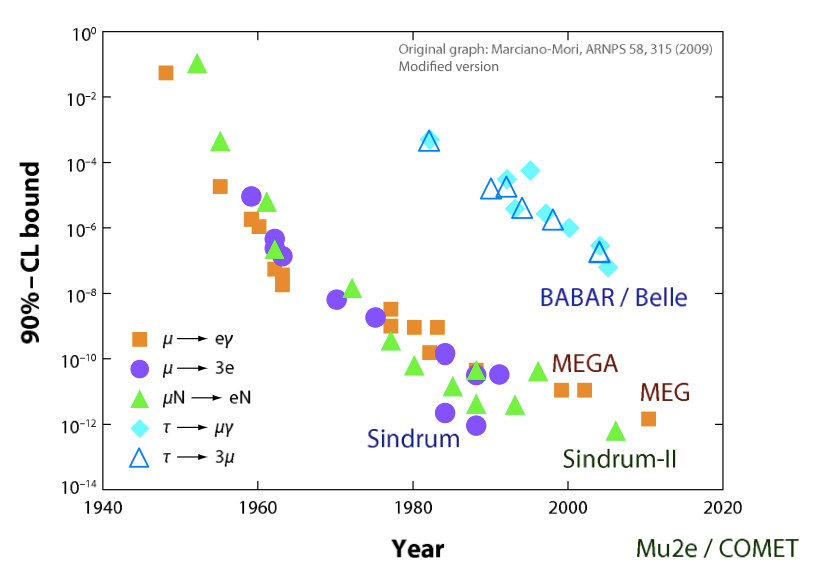
\includegraphics[width=0.8\textwidth]{Introduction/figs/LFV.png}
\caption{Summary of limits set in lepton flavour violation searches~\cite{Marciano:2008zz}.}
\label{fig:LFV_decay}
\end{figure}
 